%\pagebreak
\section*{Task \#5: Distributed Secure State Estimation of CPSs}

\subsection*{Brief theoretical introduction}
The framework in which CPSs are located is intrinsically \textbf{distributed}, for this reason we move in the direction of \textit{fusion center removal} and the use of a distributed approach also for computation; this is done by using \textbf{distributed algorithms} which requires the devices of the CPS modeled as a multi-agent systems to 
%The motivation for \textbf{decentralization} is quite practical: a large number of cheap interconnected devices is better than few expensive devices. In this part we refer to a general CPS as a \textbf{multi-agent system}, in a nutshell a collection of devices which cooperate in order to reach a \textbf{common goal}, which for our purposes is the \underline{secure state estimation (SSE) of a dynamical system}.
cooperate, in the sense that they have to exchange some information through a communication network which is modeled by a digraph. 
Important results on \textbf{Consensus algorithm} guide us in the choice of the type of information to be shared: the local estimate $x^{(i)}(k)$ of the state. Under certain condition by iterating the computation of a \textbf{local quantity}, a global estimation $x^*$, equal for all the agents (the consensus), can be reached.
The ideas on which Consensus algorithm is based can be exploited for the minimization of composite convex functionals like the Least-Squares and the LASSO one, which is used for our purposes.
This brings us to a \textbf{distributed context} in the sense that if each node has got its own part of the composite convex functional, this is suitable to be used to compute and update local estimate also using the information sent by the nodes in its neighbourhood. This is the idea on which algorithms like the Distributed Gradient Descent (for the distributed solution of LS) and Distributed ISTA (for distributed solution of LASSO) are formulated.\\
The \textbf{objective of this task} is instead to solve the \textit{RSS-Fingerprinting based target localization problem} in a distributed way using the DIST algorithm.
 
%----------------------------------------------
\vspace{-0.3cm}
\subsection*{Algorithm}
The algorithm, whose steps are summarized in the following, aims to find a solution to the problem (\ref{eq:LASSO}) in a distributed way. Each agent has its own $y_i$ and $A_i$ which is the $i$-th row of the matrix $A$.

\begin{algorithm}
    \caption{Distributed Iterative Shrinkage/Thresholding algorithm (\textbf{DISTA})}
    \begin{enumerate}
        \itemsep-0.3em
        \item \textbf{Initialization}: $x^{(i)}(0)\in \mathbb{R}^n$ (eg. $x^{(i)}(0)=0$) 
        \item For $k=1,..., T_{max}$
        \item For each agent $i=1,...,q \quad$ 
        $x^{(i)}(k+1) = \mathbb{S}_{\lambda\tau} 
            \bigg[ 
                \sum_{i=1}^q Q_{i,j}x^{(j)}(k) +
                \tau A_i^T(y_i-A_ix^{(i)}(k))
            \bigg]$
    \end{enumerate}
    \vspace{-0.4cm}
\end{algorithm}
\noindent
$\mathbb{S}_{\lambda\tau}$ is the \textbf{Shrinkage/Thresholding operator} used also in the previous tasks, while the matrix $Q$ is the \textbf{stochastic matrix} associated to the directed graph through which the interconnection among the agents is modeled. The conditions under which such agents can reach the consensus can be verified by analyzing the eigenvalues of such a matrix according to the \textbf{Perron-Frobenius Theorem}. Moreover if the matrix $Q$ has the properties required by such a theorem and it is \textit{doubly stochastic} it reaches the average consensus, which is an even stronger result.\\
About the \textbf{cell grid discretization} and the structure of the solution, the setting is the same than the other tasks (both the state to estimate and the attacks are sparse).
%----------------------------------------------
\vspace{-0.3cm}
\subsection*{Analysis and Results}
In the following four different graph topologies with different connectivity properties have been proposed. For each one, the \textbf{spectral properties} and \textbf{the convergence} is analysed. In particular is useful to recall that: 
\begin{enumerate}
    \itemsep-0.5em
    \item A matrix is said to be (row) \textbf{stochastic} if the sum of the element for each row is equal to one; \textbf{doubly stochastic} if even the sum of the entries on the columns is equal to one; 
    \item The agents which communicate according to a certain $Q$ matrix \textbf{reach the consensus} if {$\lambda_1=\lambda_{PF}=1>\vert \lambda_2 \vert \ge ... \ge \vert \lambda_q$} 
    \item The convergence of the consensus algorithm is determined by the \textbf{essential spectral radius} which is the \textbf{second largest eigenvalue in magnitude}.  
\end{enumerate}

\begin{figure}[h]\label{fig:Topologies}   
    \vspace{-1cm}
    \centering 
    \subfigure[$Q_4$]
    {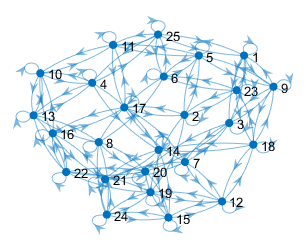
\includegraphics[scale=0.67]{img/Q4.png}}
    \subfigure[$Q_8$]
    {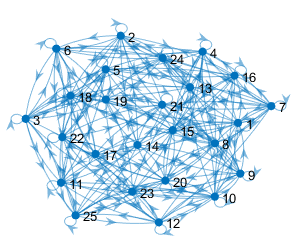
\includegraphics[scale=0.67]{img/Q8.png}}
    \subfigure[$Q_{12}$]
    {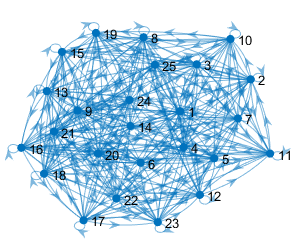
\includegraphics[scale=0.67]{img/Q12.png}}
    \subfigure[$Q_{18}$]
    {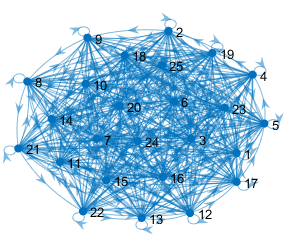
\includegraphics[scale=0.67]{img/Q18.png}}
    \caption{Topologies on which the analysis is conducted}
    \label{fig:Graphs}
\end{figure}
\begin{table}[h]\label{table:analysis}
    \centering
    \begin{tabular}{| p{3.5cm} | p{5.5cm} |p{2cm} |p{5cm} | }
        \hline
        \textbf{TOPOLOGY (Q)}&\textbf{EIGENVALUES $\vert \lambda_i \vert$}&\textbf{\texttt{esr}(Q)}&\textbf{CONVERGENCY TIME}\\
        \hline
        {\Large  $Q_4$}&{\small
            0.0450 ...
    0.7785
    \underline{1.0000}
        }&      {0.7785}&       { 10278}\\
        \hline
        {\Large  $Q_8$}&{\small
            0.0058 ...
    0.4964
    \underline{1.0000}
        }&    { 0.4964}&{ 10498}\\
        \hline
        {\Large $Q_{12}$}&{\small
            0.0053 ...
    0.3701
    \underline{1.0000}
        }&  { 0.3701}&{  10401}\\
        \hline
        {\Large  $Q_{18}$}&{\small
            0.0096 ...
        0.2196
        \underline{1.0000}}&   { 0.2196}&{10637}\\
        \hline
    \end{tabular}
    \caption{Main results for the analysis of the four topologies}
\end{table}

\noindent
The four matrices associated with the proposed topologies in Figure (2) have eigenvalues which satisfy the Perron-Frobenius Theorem since all are in magnitude less than $\lambda_{PF}=1$, then they reach consensus. Moreover, since the matrices are even \textbf{doubly stochastic} the system reaches the \textit{average consensus}.
About the \textbf{convergency} we can state that a smaller value for the essential spectral radius is associated with an higher number of needed iterations to converge. This information is summarized in the Table (2) 

\begin{wrapfigure}{r}{0.35\linewidth}
    \vspace{-0.3cm}
    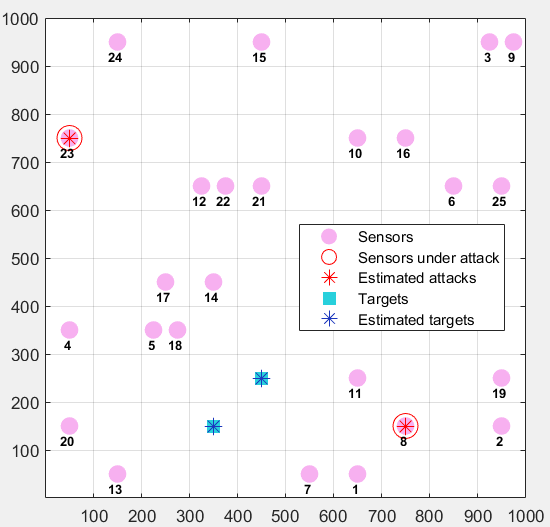
\includegraphics[width=0.9\linewidth]{img/Room.png} 
    \caption{Sensors, Target, estimates}
    \label{fig:Room}
\end{wrapfigure}
Furthermore, The algorithm has a \textbf{good accuracy} since the estimate for both the support for the target position (progressive number of the cells) and sensors under attack are correct, the Figure (\ref{fig:Room}) shows this result.
Another consideration can be done on the entries of the stochastic matrices. In particular, trying to change the magnitude of the entries $Q_{ij}$ there are not big differences on the convergency time. However in some situtions can be useful taking into account the weight of the edges. For example, let us suppose that on a link there is an attack in the sense that a certain sensor spread the measurement of the state corrupted by a quantity $a$, in that situation can be crucial - for the Secure State Estimation - the reduction of the quantity $Q_{ij}$ associated with the link under attack. [Note that in Table (\ref{table:analysis}) only a subset of the eigenvalues have been reported, the first one, the second one and the last one, they are in increasing order of magnitude].
%----------------------------------------------